\documentclass{optica-article}
\journal{opticajournal}
\articletype{Research Article}
% XeTeX equivalent of the template's Helvetica family; layout is unchanged.
\usepackage{iftex}
\ifXeTeX
\usepackage{fontspec}
\setsansfont{texgyreheros-regular.otf}[BoldFont=texgyreheros-bold.otf,ItalicFont=texgyreheros-italic.otf,BoldItalicFont=texgyreheros-bolditalic.otf]
\fi
\usepackage{booktabs}
\let\openbox\relax
\usepackage{amsthm}
\usepackage{lineno}
\linenumbers
\newtheorem{theorem}{Theorem}
\newtheorem{proposition}[theorem]{Proposition}
\newtheorem{corollary}[theorem]{Corollary}
\newcommand{\Cg}{\mathcal C_g}
\newcommand{\Dg}{\mathcal D_g}
\newcommand{\B}{\mathcal B}
\newcommand{\ip}[2]{\langle #1,#2\rangle}
\newcommand{\norm}[1]{\lVert#1\rVert}
\begin{document}
\title{Certified illumination-test counts: limits imposed by spectral regularity and measurement tolerance}
\author{Shankhya Debnath\authormark{1,*}}
\address{\authormark{1}Department of Printing Technology, Regional Institute of Printing Technology, Kolkata, India}
\email{\authormark{*}shankhya@riptkolkata.org}
\begin{abstract*}
How many illumination tests guarantee a prescribed color-mismatch limit under other lighting? For a fixed CIE library and continuous passive reflectances with slope at most $0.0355\,\mathrm{nm}^{-1}$, five tests are necessary and sufficient for a normalized XYZ infinity-norm limit of 0.02 over a positive tolerance interval. Exact counterexamples defeat every smaller selection. Continuous certificates enclose the boundary between precision and spectral regularity and prove that the count survives quantified reflectance-model and illumination errors. A calibrated affine predictor gives a supporting optimal-recovery interpretation. Rational verification and independent MATLAB checks establish these results for the declared continuous model.
\end{abstract*}
\noindent\textit{Author-review draft. Author preparation of the narrative is required before submission under the journal's AI-text policy.}

\section{Introduction}
Two objects that match under one light can differ under another. Additional illumination tests constrain this ambiguity, but how many are sufficient? We ask for the smallest selection from a declared library that bounds deployment mismatch for every pair in a specified reflectance class. An upper certificate establishes sufficiency. Proving a minimum also requires counterexamples covering every smaller selection.

Metameric reflectance construction and multiple-illuminant matching are established problems~\cite{worthey,burns}. Metamer sets have been used for reflectance estimation~\cite{morovic2006}; set-theoretic methods combine measurement consistency with physical and smoothness constraints~\cite{sharma}. Smoothness affects metamer-mismatch regions~\cite{stiebel}, and operator formulations describe the information lost in color formation~\cite{morovic2026a,morovic2026b}. Illumination and filter design also support spectral recovery~\cite{park,fu,niu}. These studies motivate the present problem, whose objective is a guaranteed maximum coordinate error for an entire function class. Illuminant-induced mismatch measures based on response-set volumes or perceptual shifts address related, different objectives~\cite{esposito}.

Classical optimal recovery and robust experiment design already treat worst-case information, bounded errors, and model uncertainty~\cite{novak,tanaskovic,ettehad,foucart}. We use their supporting principles. The contribution here is the evaluated count and precision boundary for a continuous color model, together with explicit uncertainty regions that preserve the minimum count. At the chosen spectral slope, every four-light selection fails even with exact tests, while all five lights succeed with positive tolerance. Once all five are retained, increased precision more than doubles the certified critical-slope range relative to tolerance 0.002. The result concerns the stated library, observer, metric, and spectral class.

\section{Testing problem and spectral model}
Let $I=[380,780]$ nm and $f_X,f_Y,f_Z$ be the CIE 1931 two-degree color-matching functions. Define
\begin{equation}
 Z_E=\int_I E f_Y>0,\qquad a_{E,c}=\frac{E f_c}{Z_E},\qquad
 A_Er=(\ip{a_{E,c}}r)_{c=X,Y,Z},                 \label{eq:response}
\end{equation}
where $\ip kr=\int_I k(\lambda)r(\lambda)\,d\lambda$. White has $Y=1$ under each light; XYZ weights are one. No chromatic adaptation or perceptual transformation is applied. The CIE tables~\cite{ciexyz,ciea,cied65,ciefl} define the nominal continuous model: each SPD and matching function is separately interpolated linearly between its 1 nm values. Their product, and the normalizer $Z_E$, are integrated exactly. The resulting kernels are piecewise quadratic; physical lamps and observers need not follow this interpolation.

The passive reflectance class and its exact difference class are
\begin{align}
 \Cg&=\{r:I\to[0,1]:\operatorname{Lip}(r)\leq g\},\nonumber\\
 \Dg=\Cg-\Cg&=\{d:|d|\leq1,\ \operatorname{Lip}(d)\leq2g\}. \label{eq:class}
\end{align}
Here $g$ has units $\mathrm{nm}^{-1}$. The class is compact in the uniform norm, convex, and symmetric about $1/2$. The reverse difference-class inclusion follows by setting $r_\pm=(1\pm d)/2$.

The test library $\mathcal L$ contains A, D65, FL2, FL7, and FL11. The deployment family $\mathcal E$ contains FL3, FL8, and FL12. One test measures all three XYZ coordinates under one constituent light. Stack the selected test responses into $M_T$ and the deployment responses into $Q:C(I)\to\mathbb R^9$. Define
\begin{equation}
 \B_g(T;\boldsymbol\delta)=
 \max_{\substack{d\in\Dg\\\norm{A_i d}_\infty\leq\delta_i,\ i\in T}}
       \norm{Qd}_\infty.                                \label{eq:B}
\end{equation}
For common tolerance $\delta$ and deployment limit $\tau=0.02$, write
\begin{align}
 n_g(\delta)&=\min\{|T|:T\subseteq\mathcal L,\ \B_g(T;\delta)\leq\tau\},\nonumber\\
 G(\delta)&=\sup\{g\geq0:\B_g(\mathcal L;\delta)\leq\tau\}. \label{eq:countG}
\end{align}
Set $n_g=\infty$ if no selection succeeds. Increasing $g$ or $\delta$ cannot reduce $\B_g$; adding tests cannot increase it. The $\delta_i$ are pairwise acceptance tolerances. Additive measurement-error bounds enter separately in Section~\ref{sec:prediction}.

\section{Continuous certificates and counterexamples}
\subsection{Upper bounds}
Write the rows of $M_T$ as $m_i$ and one row of $Q$ as $q$. Choose multipliers $v_i$ and an absolutely continuous function $p$ with $p(380)=p(780)=0$. Put
\begin{equation}
 u=q-\sum_i v_i m_i,\qquad R=\int_I|u+p'|,\qquad
 P\geq\int_I|p|,\qquad N=\sum_i|v_i|.                    \label{eq:certificate}
\end{equation}
\begin{proposition}[Continuous certificate]\label{prop:dual}
If $d\in\Dg$ and $|\ip{m_i}d|\leq\delta_i$, then
\begin{equation}
 |\ip qd|\leq R+2gP+\sum_i|v_i|\delta_i.                 \label{eq:dual}
\end{equation}
\end{proposition}
\begin{proof}
Integration by parts gives
$\ip qd=\sum_i v_i\ip{m_i}d+\ip{u+p'}d+\int_I p d'$.
The endpoint terms vanish. Apply $|d|\leq1$ and $|d'|\leq2g$ almost everywhere.
\end{proof}
One certificate per target coordinate bounds $\norm{Qd}_\infty$. This support inequality has the residual-functional structure used in optimal recovery~\cite{foucart,ettehad}; its purpose here is to certify the numerical testing results.

On a wavelength cell $[a,a+h]$, $u$ is quadratic. Specifying endpoint values of $p$ and setting
\begin{equation}
 p'=c-u,\qquad
 c=\frac{p(a+h)-p(a)+\int_a^{a+h}u}{h}                  \label{eq:flux}
\end{equation}
produces a continuous piecewise-cubic $p$, with cell contribution $h|c|$ to $R$. Write the cubic as $p=\sum_{k=0}^3 b_k B_{k,3}$ in the Bernstein basis. Positivity gives
$\int_a^{a+h}|p|\leq(h/4)\sum_{k=0}^3|b_k|$.
Dyadic subdivision tightens this bound. Bernstein bounds are established numerical tools~\cite{ricciardi}; here they provide a rational upper enclosure for $P$.

Numerical optimization supplies candidate multipliers and fluxes. The checker treats saved coefficients and decimal CIE values as exact rationals, reconstructs Eq.~\eqref{eq:flux}, and verifies all residual and integral bounds. A solver tolerance or a successful wavelength-grid calculation alone does not establish the continuous guarantee.

\subsection{Lower bounds and the precision boundary}
A stored piecewise-linear difference $d$ gives a lower certificate. Nodal amplitudes and interval slopes verify membership in $\Dg$ everywhere. Integrating its product with each quadratic kernel gives exact responses. For each four-light selection, rational elimination enforces twelve zero test responses; scaling enforces the amplitude and slope bounds. Every smaller subset lies inside a four-light selection, so five witnesses cover all 31 selections with fewer than five lights, including the empty set.

For common tolerance, each upper certificate gives $R_j+2gP_j+\delta N_j\leq\tau$. The bank contains 81 original certificates and nine verified convex combinations for matching target coordinates. Its sufficient slope envelope is
\begin{equation}
 G_-(\delta)=\min_{c}\max_{j:q_j=q_c}
       \frac{\tau-R_j-\delta N_j}{2P_j},                \label{eq:lowerenv}
\end{equation}
using its nonnegative portion; all stored $P_j$ are positive. Failure witnesses give an upper envelope $G_+$. Witnesses whose targets exceed $\tau$ in the same signed coordinate may be combined convexly: their amplitude, slope, and test bounds combine convexly, and failure remains strict. This yields continuous failure segments. Exact intersections of these segments and the certificate envelopes establish
$G_-\leq G\leq G_+$ on $0\leq\delta\leq0.002$.
Combining witnesses with different failing coordinates would not justify that conclusion. A bracket endpoint obtained from strict failure also need not itself be a strict-failure point.

\section{Sharp count and the value of precision}
\begin{theorem}[Minimum constituent count]\label{thm:count}
For $g=0.0355\,\mathrm{nm}^{-1}$ and $\tau=0.02$,
\begin{equation}
 n_g(\delta)=5\quad\text{for }0\leq\delta\leq0.000181293988. \label{eq:five}
\end{equation}
Every smaller selection fails even at $\delta=0$.
\end{theorem}
\begin{proof}
Nine full-library certificates satisfy Eq.~\eqref{eq:dual} at the upper tolerance in Eq.~\eqref{eq:five}; monotonicity gives sufficiency throughout the interval. Each witness in Table~\ref{tab:four} belongs to $\Dg$, matches all twelve selected test coordinates exactly, and exceeds $\tau$ in deployment. Their subset coverage proves necessity for all 31 smaller selections at every nonnegative tolerance.
\end{proof}

\begin{table}[t]
\centering
\caption{Exact-test witnesses for all four-light selections. Each pair matches the other four lights exactly and has individual slopes below $0.0355\,\mathrm{nm}^{-1}$. Lower bounds are rounded downward.}
\label{tab:four}
\begin{tabular}{lc}
\toprule
Omitted light & Deployment mismatch lower bound\\
\midrule
FL11 & 0.225987634044\\
FL7  & 0.025614387784\\
FL2  & 0.022987792057\\
D65  & 0.021836307236\\
A    & 0.028894428339\\
\bottomrule
\end{tabular}
\end{table}

Figure~\ref{fig:witness} shows the witness with the smallest failure margin. These are constructed spectra, not measured materials. Increasing the precision of its four selected tests cannot distinguish the pair. At $\delta=0.0001$, all five tests give the universal upper bound $0.019183170792$. A full-library witness proves failure by $\delta=0.000183138235$. The largest successful tolerance at this slope is therefore enclosed between $0.000181293988$ and $0.000183138235$.

\begin{figure}[t]
\centering
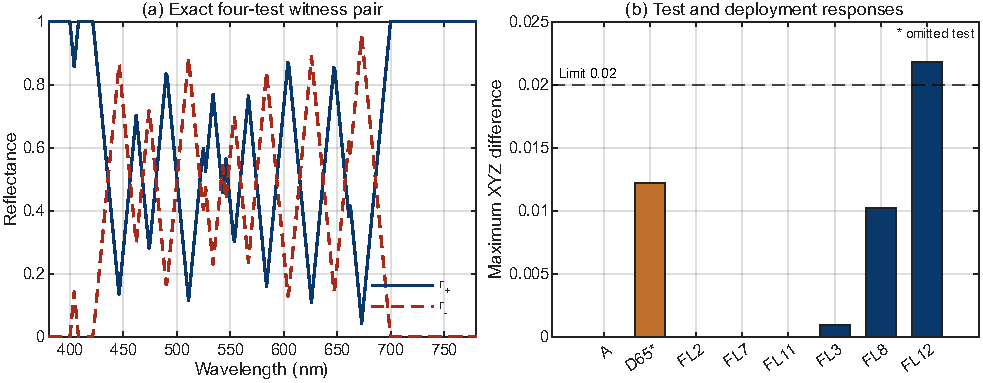
\includegraphics[width=\textwidth]{witness.pdf}
\caption{Exact-matching counterexample for A, FL2, FL7, FL11. (a) The continuous passive spectra $r_\pm=(1\pm d)/2$. (b) Maximum XYZ difference under each light. Selected test responses are exactly zero; the deployment mismatch exceeds 0.02. D65 is the omitted candidate test. MATLAB plots stored records; plotting code was prepared with OpenAI Codex assistance.}
\label{fig:witness}
\end{figure}

With all five tests retained, the critical-slope brackets are
\begin{align}
 G(0)&\in[0.039324263178,\ 0.039394217170],\nonumber\\
 G(0.002)&\in[0.018486923133,\ 0.018546626551]
                         \quad(\mathrm{nm}^{-1}).       \label{eq:critical}
\end{align}
The ratio between the first lower bound and the second upper bound exceeds 2.12. Figure~\ref{fig:frontier} gives the intervening enclosure. Its maximum unresolved width is at most $0.001104210242\,\mathrm{nm}^{-1}$, so the predeclared uniform resolution target of $0.001\,\mathrm{nm}^{-1}$ was missed. The tolerance bracket at $g=0.0355$ also missed its tighter resolution target. These gaps concern boundary precision; Eq.~\eqref{eq:five} proves an exact count on its stated interval. The calculations followed successive bounded investigations, with their development history retained in the repository.

\begin{figure}[t]
\centering
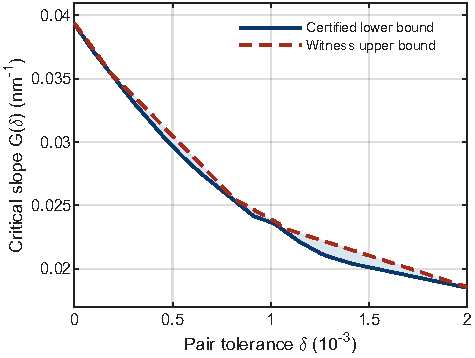
\includegraphics[width=0.86\textwidth]{frontier.pdf}
\caption{Continuous enclosure of the full-library critical slope $G(\delta)$. The lower envelope certifies success; the upper envelope follows from strictly failing spectra. The intervening band remains unresolved. The curves use verified affine segments, not interpolation of sampled optima. MATLAB plotting code was prepared with OpenAI Codex assistance.}
\label{fig:frontier}
\end{figure}

\section{Stability of the minimum count}
\subsection{Reflectance-model and normalized-kernel errors}
Let $\Cg^\rho$ contain passive continuous $r$ within uniform distance $\rho$ of some $r_0\in\Cg$. Actual spectra need not satisfy the nominal slope bound. An actual difference $d$ then has $|d|\leq1$ and a $d_0\in\Dg$ with $\norm{d-d_0}_\infty\leq2\rho$. Write actual kernels as $m_i'=m_i+e_i$ and $q'=q+f$, with uniform $L^1$ bounds $\norm{e_i}_1,\norm f_1\leq\mu$. Acceptance is measured using these actual kernels. With $U=\int_I|u|$, a certificate gives
\begin{equation}
 |\ip{q'}d|\leq R+2gP+\delta N+(1+N)\mu+2\rho U.        \label{eq:robust}
\end{equation}
Indeed, decompose the target into
$\sum_i v_i\ip{m_i'}d+\ip u{d_0}+\ip u{d-d_0}+\ip{f-\sum_i v_i e_i}d$.
Integration by parts bounds the nominal term; the other terms use actual test acceptance, uniform model distance, and passivity. Keeping the combined residual $U$ uses the classical residual-norm principle~\cite{foucart}. The smaller quantity $R$ cannot replace $U$, since $d-d_0$ has no derivative bound.

At $g=0.0355$, $\delta=0.0001$, and $\tau=0.02$, the nine inequalities certify the region
\begin{equation}
 \frac{\mu}{0.000073935629}+\frac{\rho}{0.005633164098}\leq1,
 \qquad\mu,\rho\geq0.                                 \label{eq:kernelregion}
\end{equation}
The denominators are rounded inward. Necessity holds for every allowed kernel realization: a nominal exact witness has selected actual responses at most $\mu\norm d_\infty$ and actual deployment magnitude at least $t-\mu\norm d_\infty$, where $t$ is its nominal target magnitude. Throughout Eq.~\eqref{eq:kernelregion}, these bounds respectively lie below $\delta$ and above $\tau$. The same five witnesses therefore exclude all smaller selections in the perturbed problem.

\subsection{Shared illuminant errors and normalization}
To retain the dependence among XYZ channels, suppose each light satisfies
\begin{equation}
 E'=a(E+\Delta E),\qquad a>0,\qquad
 |\Delta E(\lambda)|\leq\kappa E(\lambda),\quad0\leq\kappa<1. \label{eq:spd}
\end{equation}
The observer is fixed, and each response uses its actual white-$Y$ normalizer. Gain $a$ cancels. The continuous shape condition prohibits leakage where $E=0$. For test light $\ell$, put
$s_\ell=\sum_c v_{\ell c}m_{\ell c}$ and
$S=\int_I q+\sum_\ell\int_I|s_\ell|$.
The XYZ kernels are nonnegative. If $z_\ell=\int\Delta E_\ell f_Y/Z_\ell$, then $|z_\ell|\leq\kappa$ and
\begin{equation}
 \ip{s_\ell}d=(1+z_\ell)\sum_c v_{\ell c}\ip{m_{\ell c}'}d
 -\int_I\frac{\Delta E_\ell}{Z_\ell}\Bigl(\sum_c v_{\ell c}f_c\Bigr)d. \label{eq:block}
\end{equation}
The two terms are bounded by $(1+\kappa)\delta\sum_c|v_{\ell c}|$ and $\kappa\int|s_\ell|$. Including the target denominator gives
\begin{equation}
 |\ip{q'}d|\leq
 \frac{R+2gP+\delta N+\kappa(\delta N+S)+2\rho U}{1-\kappa}. \label{eq:spdrobust}
\end{equation}
The resulting nine affine inequalities certify
\begin{equation}
 \frac{\kappa}{0.000103842397}+\frac{\rho}{0.005633164098}\leq1,
 \qquad\kappa,\rho\geq0.                               \label{eq:spdregion}
\end{equation}
For a nominal exact witness, let $I_i=\int m_i|d|$ and $I_q=\int q|d|$. Its actual tests are at most $\kappa I_i/(1-\kappa)$ and its target magnitude is at least $(t-\kappa I_q)/(1+\kappa)$. Exact integration bounds all selected witness tests by $0.000055671797$ and all five deployment witnesses below by $0.021803184702$ throughout Eq.~\eqref{eq:spdregion}. Hence all 31 smaller selections fail for every allowed SPD realization.

\begin{corollary}\label{cor:robustcount}
At $g=0.0355\,\mathrm{nm}^{-1}$, $\delta=0.0001$, and $\tau=0.02$, the minimum constituent count remains five throughout either Eq.~\eqref{eq:kernelregion} or Eq.~\eqref{eq:spdregion}, under its respective uncertainty model.
\end{corollary}

\begin{figure}[t]
\centering
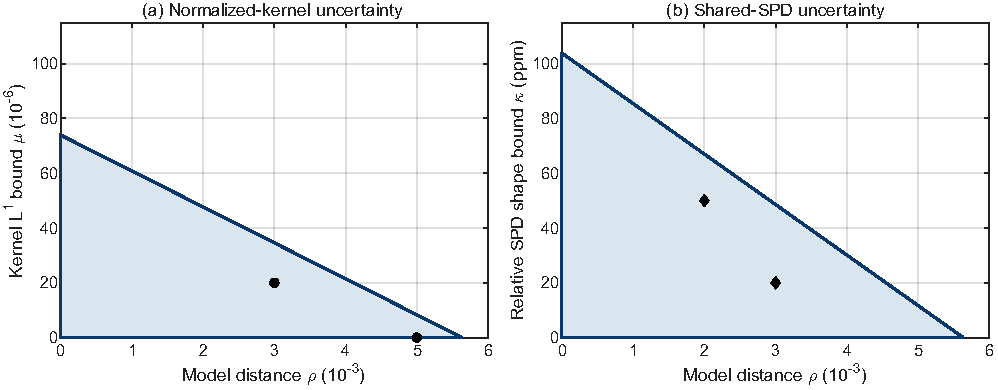
\includegraphics[width=\textwidth]{stability.pdf}
\caption{Sufficient regions preserving the five-test minimum. (a) Uniform model distance $\rho$ and normalized-kernel $L^1$ error $\mu$. (b) Model distance and relative SPD-shape error $\kappa$, with actual white normalization. The two vertical axes describe different uncertainties. Markers denote verified examples in the data package. Maximal physical uncertainty regions are unknown. MATLAB plotting code was prepared with OpenAI Codex assistance.}
\label{fig:stability}
\end{figure}

Figure~\ref{fig:stability} shows both regions. In the kernel model, $\mu=0.00002$ and $\rho=0.003$ give a five-test upper bound of $0.019839138517$. Every smaller selection has a lower bound of $0.021816307342$. In the shape model, $\kappa=0.00005$ and $\rho=0.002$ give respective bounds of $0.019866473729$ and $0.021820357914$. The shape-only allowance is approximately 103.84 parts per million. These are sufficient mathematical bounds; experimental lamp specifications require separate validation. Checking all 90 stored certificates did not improve the intercepts by selecting another individual certificate. That finite-bank result leaves open improvements from new certificates or a different analysis.

\section{Supporting prediction interpretation}\label{sec:prediction}
Fix the operators and observations $y=M_Tr+\eta$, with independently admissible errors $\norm{\eta_i}_\infty\leq\varepsilon_i$. For each feasible $y$, the response set
$K_y=Q\{r\in\Cg:y-M_Tr\in N_{\boldsymbol\varepsilon}\}$ is compact. Its coordinatewise range midpoints give a smallest enclosing ball in the infinity norm, of radius half its diameter. Minimizing over arbitrary prediction rules $\Phi$ therefore gives the classical identity
\begin{equation}
 E_\infty^*(T;\boldsymbol\varepsilon)
 :=\inf_\Phi\sup_{r\in\Cg,\,\eta\in N_{\boldsymbol\varepsilon}}
 \norm{\Phi(M_Tr+\eta)-Qr}_\infty
 =\tfrac12\B_g(T;2\boldsymbol\varepsilon).              \label{eq:recovery}
\end{equation}
The factor two follows because two spectra share an observation exactly when their selected responses differ by at most $2\varepsilon_i$. For another additive noise set $N$, the overlap condition is $M_T(r-s)\in N-N$. A predictor constrained to return the response of an admissible reconstructed spectrum may have a larger radius. In Euclidean norm, half the diameter is generally only a lower bound; nonlinear perceptual differences do not inherit Eq.~\eqref{eq:recovery}.

Convex symmetry of the class and noise permits classical scalar affine optimality~\cite{novak,ettehad}; applying it to each target coordinate gives affine optimality for the infinity-norm problem. The supplied predictor is certified, without a claim that its coefficients attain the exact minimax value. Its nine multiplier rows form $V\in\mathbb R^{9\times15}$. With white estimates $w_M,w_Q$ within coordinatewise error $\gamma$ of $M'1,Q'1$, use
\begin{equation}
 \widehat z=V(y-w_M/2)+w_Q/2.                            \label{eq:predictor}
\end{equation}
The information includes target white responses. White calibration requires exposures beyond the counted sample tests. To bound the error, write $r=1/2+x$ and $r_0=1/2+x_0$. Passivity gives $|x|,|x_0|\leq1/2$, while $\operatorname{Lip}(x_0)\leq g$ and $\norm{x-x_0}_\infty\leq\rho$. Applying the certificate to each row gives
\begin{equation}
 |\widehat z_j-(Q'r)_j|\leq R/2+gP+\varepsilon N+\rho U
                       +(\mu+\gamma)(1+N)/2.           \label{eq:prederror}
\end{equation}
At $\varepsilon=0.00005$, error is at most 0.01 when
$(\mu+\gamma)/0.000073935629+\rho/0.005633164098\leq1$.
Using nominal whites alone gives $\gamma\leq\mu$, which charges $2\mu$ in this inequality. The nominal upper error is $0.009591585396$; every smaller selection has worst-case error at least $0.010918153618$.

At $(\mu,\gamma,\rho)=(0.00002,0,0.003)$, the five-test upper error is $0.009919569259$. Every smaller selection has error at least $0.010908153671$. The witnesses admit the common central observation $M'1/2$ through opposing admissible noise, with identical calibration data. This also excludes deterministic adaptive choices of at most four constituents: follow the central-observation path and use a witness covering its final subset. The argument is specific to adversarial Cartesian bounded noise and constituent selection; it does not cover arbitrary mixture exposures, randomized expected error, or perturbed noiseless adaptive pair testing.

\section{Discussion}
The five-test result separates a shortage of information from insufficient precision. An exact-matching pair remains indistinguishable however precisely its four selected lights are measured. Adding the fifth light removes that particular obstruction and gives a universal guarantee for the stated class. With the complete library, improved precision admits substantially steeper spectra, as Eq.~\eqref{eq:critical} quantifies. The uncertainty regions show how far the count persists when actual spectra or illumination depart from the nominal assumptions.

The minimum is taken over five named constituents. It does not establish a minimum over all physical lights, sensors, normalizations, or mixture test exposures. A mixture can introduce a new measurement direction. Deployment mixtures, however, are covered: for $E=\sum_j a_jE_j$ with $a_j\geq0$ and not all zero,
$A_E=\sum_j\beta_j A_{E_j}$, where $\beta_j=a_jZ_{E_j}/\sum_k a_kZ_{E_k}$.
Convexity of the infinity norm extends the guarantee to every nonnegative mixture of the three deployment SPDs. Since this family includes its constituents, the worst mismatch is unchanged. The statement also holds for actual constituent SPDs under their specified uncertainty model.

These guarantees concern continuous mathematical classes. Dataset performance can help assess whether a class describes relevant materials, but cannot prove its universal bound. Constructed extremal spectra need not resemble typical manufactured surfaces. The tolerance 0.02 is a normalized XYZ coordinate limit, with no direct claim of perceptual equivalence. Lamp stability, observer variation, and distances from the slope class require experimental assessment before these bounds can inform instrument specifications.

The mathematical ingredients have precedents in multiple matching, convex spectral constraints, recovery theory, robust design, and Bernstein bounds. The numerical results establish a sharp constituent count and its stability, and quantify how precision limits the admissible spectral class. No speed, dataset-reconstruction, or perceptual advantage over existing methods is claimed. The unresolved frontier band and the sufficient nature of the uncertainty regions leave room for stronger certificates and sharper lower witnesses.

\section{Conclusion}
Five constituent tests are necessary and sufficient for the stated continuous CIE model at individual slope $0.0355\,\mathrm{nm}^{-1}$ and mismatch limit 0.02 over a positive tolerance interval. Exact witnesses exclude all smaller selections, even with noiseless tests. Continuous certificates quantify the benefit of precision and establish simultaneous model and illumination errors under which the count persists. The same certificates yield an explicit calibrated prediction bound.

\begin{backmatter}
\bmsection{Funding} No specific funding was received for this work.
\bmsection{Acknowledgments} OpenAI Codex assisted mathematical development, implementation, computational checks, plotting scripts, and preparation of this author-review draft. Figures are deterministic MATLAB plots of stored records. Author preparation and scientific review of the final narrative, and completion of the tool disclosure, remain required under the journal's policy.
\bmsection{Disclosures} The author declares no conflicts of interest.
\bmsection{Data availability} Source data, certificates, verification code, and figure-generation files are deposited in the associated repository~\cite{repository}, which is private during author review. Public release or reviewer access is required before submission. Original CIE data retain their attribution and license.
\end{backmatter}

% Bibliography retained from the evidence-checked R183 manuscript.
\clearpage
\begin{thebibliography}{30}
\bibitem{worthey} J. A. Worthey, ``Calculation of metameric reflectances,'' Color Res. Appl. \textbf{13}, 76--84 (1988).
\bibitem{burns} S. A. Burns, J. B. Cohen, and E. N. Kuznetsov, ``Multiple metamers: preserving color matches under diverse illuminants,'' Color Res. Appl. \textbf{14}, 16--22 (1989).
\bibitem{morovic2006} P. Morovi\v{c} and G. D. Finlayson, ``Metamer-set-based approach to estimating surface reflectance from camera RGB,'' J. Opt. Soc. Am. A \textbf{23}, 1814--1822 (2006).
\bibitem{sharma} G. Sharma, ``Set theoretic estimation for problems in subtractive color,'' Color Res. Appl. \textbf{25}, 333--348 (2000).
\bibitem{stiebel} T. Stiebel and D. Merhof, ``The importance of smoothness constraints on spectral object reflectances when modeling metamer mismatching,'' in \emph{IEEE International Conference on Computer Vision Workshops} (2017), pp. 2985--2992.
\bibitem{morovic2026a} P. Morovi\v{c} and J. Morovi\v{c}, ``Color formation as a Hilbert space operator: quotient structures and limits of metamerism,'' J. Opt. Soc. Am. A \textbf{43}, 1614--1623 (2026).
\bibitem{morovic2026b} P. Morovi\v{c} and J. Morovi\v{c}, ``Color formation as a Hilbert space operator: metamer mismatching and the limits of chromatic adaptation,'' J. Opt. Soc. Am. A \textbf{43}, 1668--1677 (2026).
\bibitem{park} J.-I. Park, M.-H. Lee, M. D. Grossberg, and S. K. Nayar, ``Multispectral imaging using multiplexed illumination,'' in \emph{IEEE International Conference on Computer Vision} (2007), pp. 1--8.
\bibitem{fu} Y. Fu, Y. Zou, Y. Zheng, and H. Huang, ``Spectral reflectance recovery using optimal illuminations,'' Opt. Express \textbf{27}, 30502--30516 (2019).
\bibitem{niu} S. Niu, G. Wu, and X. Li, ``Spectral filter selection based on human color vision for spectral reflectance recovery,'' Sensors \textbf{23}, 5225 (2023).
\bibitem{esposito} T. Esposito, M. P. Royer, and K. W. Houser, ``Measures of illuminant-induced metameric mismatch: theory, comparative analysis, and implications for application,'' Opt. Express \textbf{30}, 14686--14708 (2022).
\bibitem{novak} E. Novak and H. Wo\'zniakowski, \emph{Tractability of Multivariate Problems, Volume I: Linear Information} (European Mathematical Society, 2008), Sec. 4.2.
\bibitem{tanaskovic} M. Tanaskovi\'c, L. Fagiano, and M. Morari, ``On the optimal worst-case experiment design for constrained linear systems,'' Automatica \textbf{50}, 3291--3298 (2014).
\bibitem{ettehad} M. Ettehad and S. Foucart, ``Instances of computational optimal recovery: dealing with observation errors,'' SIAM/ASA J. Uncertain. Quantif. \textbf{9}, 1438--1456 (2021).
\bibitem{foucart} S. Foucart, ``Instances of computational optimal recovery: refined approximability models,'' J. Complexity \textbf{62}, 101503 (2021).
\bibitem{ciexyz} CIE, ``Colour-matching functions of CIE 1931 standard colorimetric observer,'' CIE dataset (2019), \url{https://doi.org/10.25039/CIE.DS.xvudnb9b}.
\bibitem{ciea} CIE, ``CIE standard illuminant A---1 nm,'' CIE dataset (2018), \url{https://doi.org/10.25039/CIE.DS.8jsxjrsn}.
\bibitem{cied65} CIE, ``CIE standard illuminant D65,'' CIE dataset (2019), \url{https://doi.org/10.25039/CIE.DS.hjfjmt59}.
\bibitem{ciefl} CIE, ``Relative spectral power distributions of illuminants representing typical fluorescent lamps,'' CIE dataset (2018), \url{https://doi.org/10.25039/CIE.DS.54hy6srn}.
\bibitem{ricciardi} L. A. Ricciardi and M. Vasile, ``Direct transcription of optimal control problems with finite elements on Bernstein basis,'' J. Guid. Control Dyn. \textbf{42}, 229--243 (2019).
\bibitem{repository} S. Debnath, ``Certified illumination testing: data and computational certificates,'' GitHub repository (2026), \url{https://github.com/shankhya/certified-illumination-testing}.
\end{thebibliography}
\end{document}
